\section{Results and Discussion}


\begin{figure}[t]
\centering
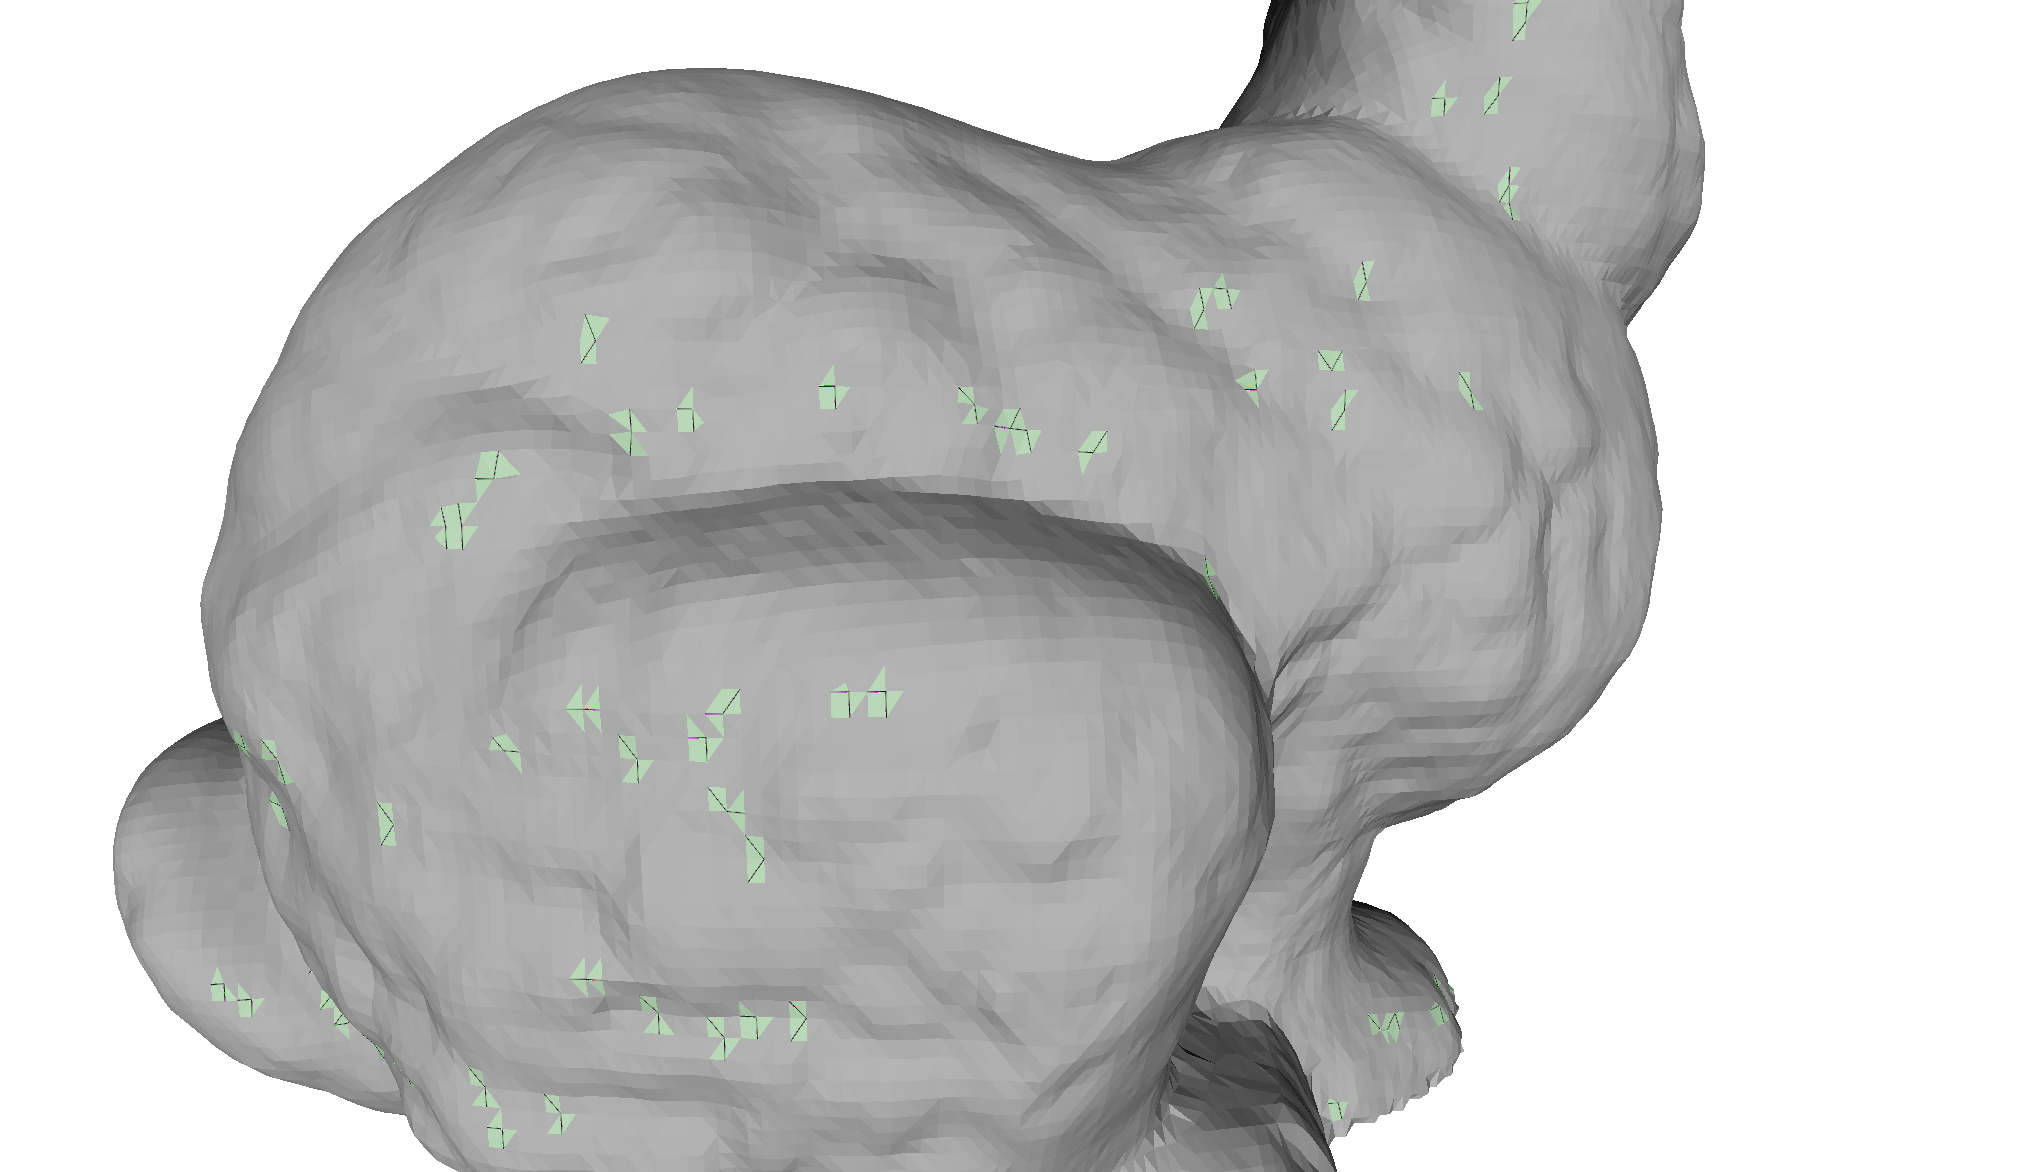
\includegraphics[width=3in]{perturb}
\caption{After perturbation, the self-union of \emph{Bunny} with QuickCSG still suffers from topology problem. The green boundary faces indicate topological deficiencies.}
%
\label{fig:boundaryedge}
\end{figure}

\begin{figure}[t]
\centering
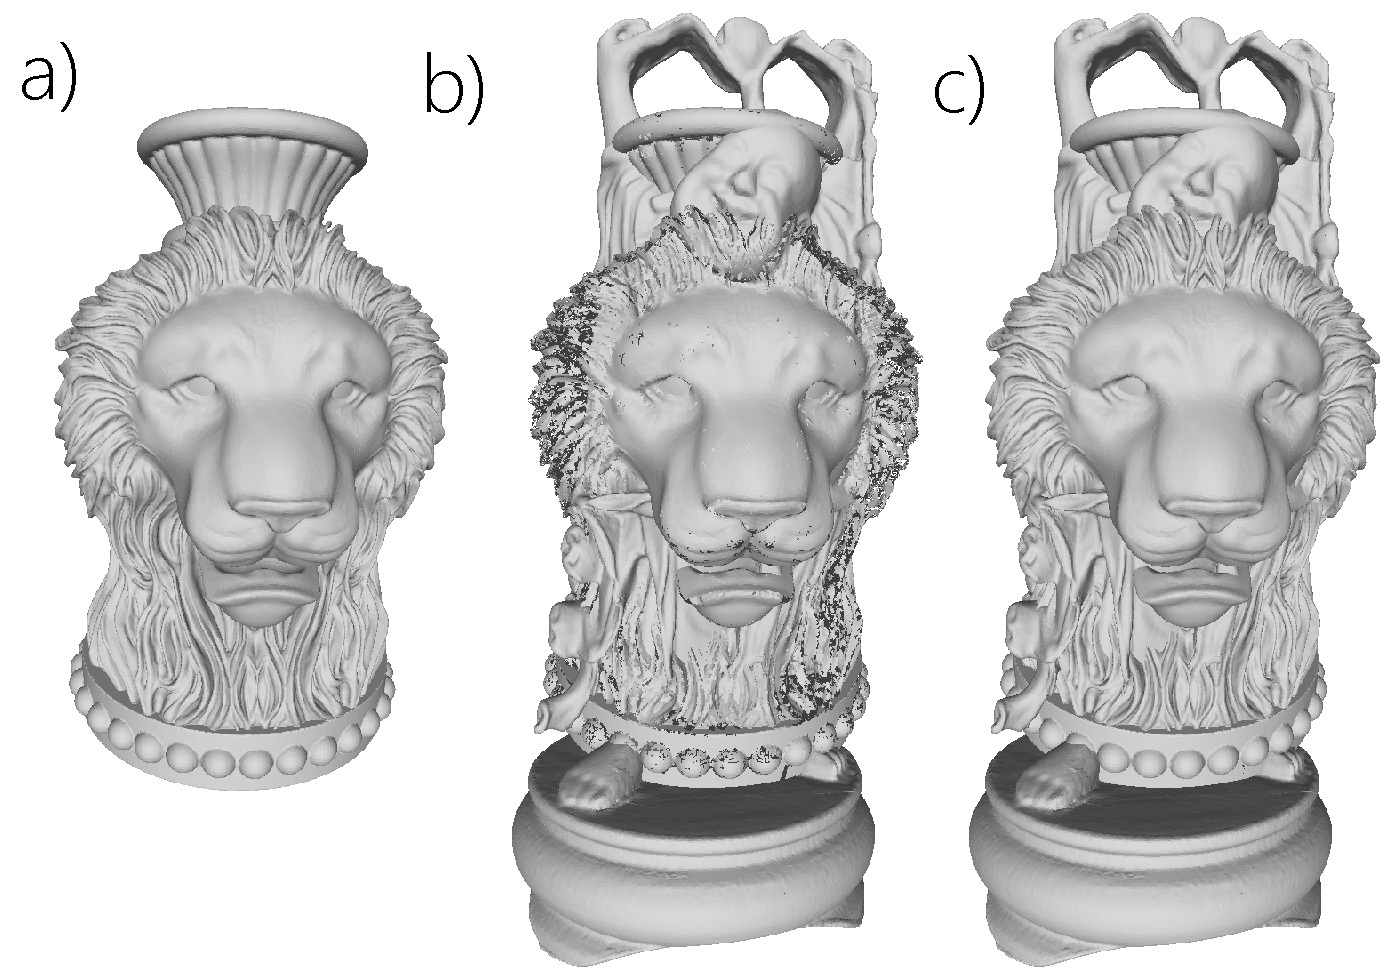
\includegraphics[width=3in]{buddalion}
\caption{ Results from $Budda\cup Lion$: a) incorrect result using CGAL, b) incorrect result using Cork, and c) correct result using our method. }
%.
\label{fig:buddalion}
\end{figure}

%We implemented the proposed method in C++ and tested a series of models on a laptop with Intel Core i5 1.5GHz CPU and 8GB RAM. To prove both the efficiency and robustness, we perform boolean evaluation on various CSGs with different complexity. We also compared our method with several previous works with available implementations, including CGAL \cite{cgal:hk-bonp3-15a}, Maya \cite{Maya2015,barki2015exact},"Cork" \cite{Cork}, "QuickCSG" \cite{douze2015quickcsg}, "Carve" \cite{Carve}, and online service of Campen and Kobbelt's plane-based method \cite{campen2010exact,WebBSP}.

We implemented our proposed method in C++, and tested a series of models on a laptop with an Intel Core i5 1.5 GHz CPU and 8 GB of RAM. To validate the efficiency and robustness of our method, we performed boolean evaluations on various CSGs with different complexities. We also compared our method with several existing methods, including CGAL \cite{cgal:hk-bonp3-15a}, Maya \cite{Maya2015,barki2015exact}, Cork  \cite{Cork}, QuickCSG \cite{douze2015quickcsg}, and Carve \cite{Carve}.



\subsection{Robustness \& Performance}



\begin{figure}[t]
\centering
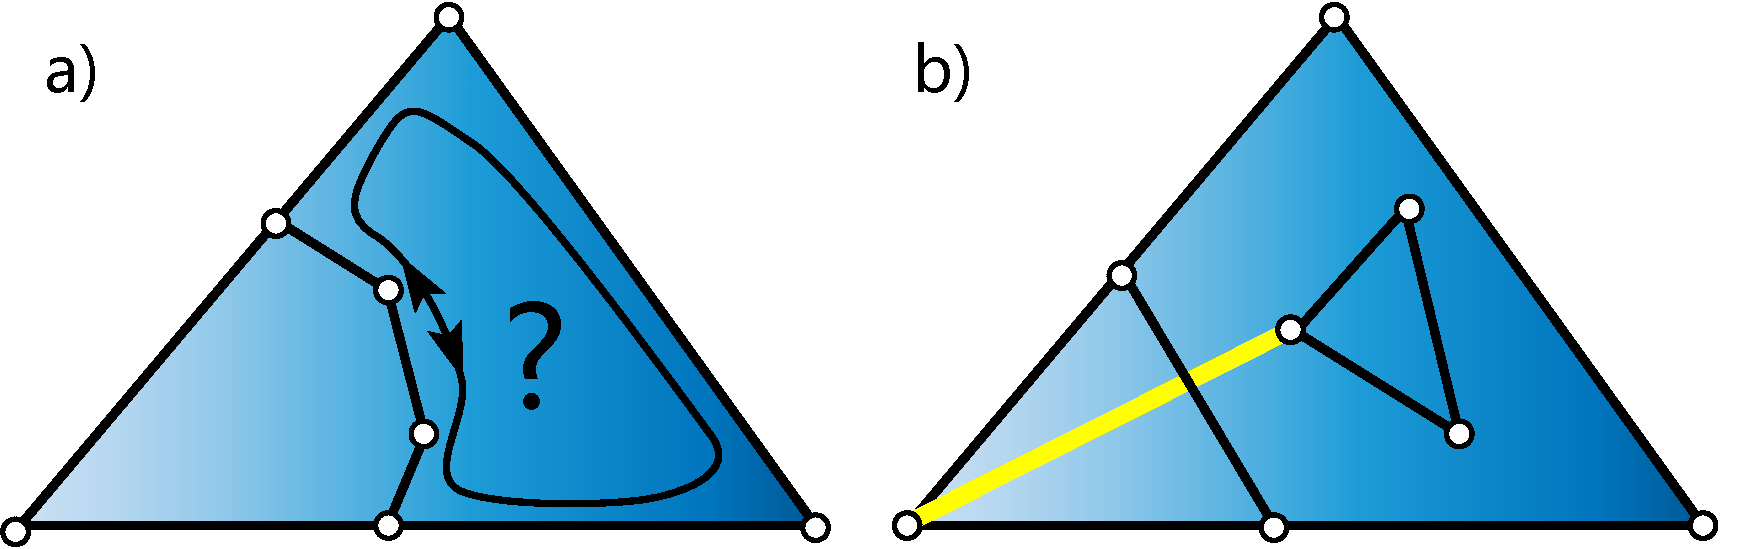
\includegraphics[width=3in]{dual}
\caption{a) There is ambiguity as to the orientation of the loop in this tess-graph. b) When there is more than one connected component in a tess-graph, auxiliary intersections (yellow line) are used to connect the components.}
\label{fig:dual}
\end{figure}



\begin{table*}[ht]
\caption{Results of self-union evaluation using different methods}
\label{tab:selfunion}
\centering
\begin{tabular}{*{8}{c|}c}%*{4}{>{\centering\arraybackslash}p{35pt}}}
\hline
{No.} & {Model} & {Face Num.} &
CGAL & Maya & Cork & Carve & QuickCSG  & Our Method
\\
\hline\hline
1 & Ball & 360  & \cmark & \cmark & \xmark & \cmark & \xmark & \cmark \\
2 & Head & 2.7k& \cmark & \cmark & \xmark & \cmark & \xmark  & \cmark\\
3 & Bunny & 70k  & \xmark & \cmark & \xmark & \cmark & \xmark  & \cmark\\
4 & Dragon & 277k & \xmark & \xmark & \xmark & \xmark & \xmark  & \cmark \\
\hline
\end{tabular}
\begin{flushleft}
\end{flushleft}
\end{table*}

\begin{table*}[ht]
\caption{Computation time statistics of binary boolean operations (seconds)}
\label{tab:performance}
\centering
\begin{tabular}{*{9}{c|}c}%*{4}{>{\centering\arraybackslash}p{35pt}}}
\hline
{No.} & {Model} & {Face Num. 1} & {Face Num. 2} &
CGAL & Maya & Cork & Carve & QuickCSG & Our Method
\\
\hline\hline
1 & Budda $\cup$ Lion & 1.08M & 400k & - & - & - & - & 3.44 & 4.30\\
2 & Dragon $\cup$ Bunny & 100k & 70k & - & - & - & - & 0.613 &1.12 \\
3 & Armadillo $\cup$ Armadillo2 & 150k & 150k & 487 & 15.4 & 7.00 & 189 & 0.746 & 1.33\\
4 & Horse $\cup$ Corpse & 145k & 499k & - & 38.6 & 12.6 & 1.52k & 0.630 & 0.980 \\
5 & Budda $\cup$ Budda2 & 1.08M & 1.08M & - & - & - & - & 4.84 & 7.73\\
\hline
\end{tabular}
\begin{flushleft}

\end{flushleft}
\end{table*}

\begin{table*}[ht]
\caption{Computation time statistics of the evaluations of large CSGs (seconds)}
\label{tab:performance2}
\centering
\begin{tabular}{*{8}{c|}c}%*{4}{>{\centering\arraybackslash}p{35pt}}}
\hline
{No.} & {Model} & {Face Num.} & {Mesh Num.} &
CGAL  & Cork & Carve & QuickCSG & Our Method
\\
\hline\hline
1 & Sprocket & 11k & 52 & 211  & - & 4.26 & 0.132 & 0.555\\
2 & Ring \& Ball & 146k & 801 & -  & - & 187 & - & 53.6\\
3 & T1 & 80k & 50 & 1.00k & 18.5 & 10.4 & 0.388 & 15.6\\
4 & T2 & 7k & 50 & 2.81k & - & 16.0 & 0.804 & 5.97 \\
%5 & H & 33k & 42 & - & - & - & 2.22 & -\\
6 & Organic & 219k & 6 & - & 14.3 & 63.1 & 0.580 & 1.74\\
%7 & 6 Budda & - & 43 & - & - & - & - & - & -\\
%8 & Serpent & - & 5 & - & - & - & - & - & -\\
\hline
\end{tabular}
\begin{flushleft}
\end{flushleft}
\end{table*}



\vspace{0.5em}
\noindent\textbf{Self-union}~~~~
Our method is unconditionally robust for regular set mesh inputs, and even extremely degenerate cases will not lead to failure. To prove this, we tested the self-union of several examples. Table . To prove that, we tested the self-union of several examples. Table  shows whether the methods tested gave valid outputs. Here, the word 'valid' means that the outputs are almost the same as the inputs. The example models \emph{Bunny} $\cap$ \emph{Dragon}  contain topological deficiencies, such as self-intersection, that cannot be processed using regular set boolean operations. Despite this, we found that our method gave good results in these cases, indicating the robustness of our method. QuickCSG and Cork failed in all cases, because they cannot process models with coplanar faces. By perturbing one of the operands, the results of QuickCSG appear visually acceptable. However, the topologies of these results are inaccurate. Hundreds of their boundary faces do not exist in the original model (Fig.  \ref{fig:boundaryedge}).


\vspace{0.5em}
\noindent\textbf{Binary boolean operations}~~~~
The most common process for CSG evaluation is to perform boolean operations in series. Although our method can evaluate multiple boolean operations simultaneously, we compared the performance of binary boolean operations to determine its efficiency. Table \ref{tab:performance} shows the evaluation times of different methods. These results show that  our method is very fast, and that it is half the speed of the fastest non-robust method, QuickCSG. Other robust methods, such as Maya and CGAL, are much slower, because they use arbitrary precision arithmetic. Moreover, these robust methods have very strict requirements for the inputs, and do not always deal well with topological deficiencies. These methods simply fail when the inputs are not valid, while our method always attempts to provide a result. With (some) very large CSGs, our method spends the most time on octree construction. This means the other stages, which involve plane-based geometry, take only a small percentage of the time. This further demonstrates the efficiency of our plane-based algorithms*.

\vspace{0.5em}
\noindent\textbf{CSGs with large number of meshes}~~~~
To identify the ability of the methods to evaluate large CSGs, we tested some CSGs with tens or hundreds of meshes. Only QuichCSG and our method can perform multiple boolean operations directly. Other methods decompose CSG trees into binary boolean operations. The computation times of robust methods like CGAL and Maya were found to be unacceptably long for large CSGs. Conversely,  our method showed good performance and stability. During our experiments, Maya gave the correct results in the first few binary boolean operations, but failed in the later ones. This demonstrates a disadvantage of incremental boolean operation methods��they can accumulate numerical errors which affect the algorithm��s stability.


\begin{figure*}[!t]
\centering
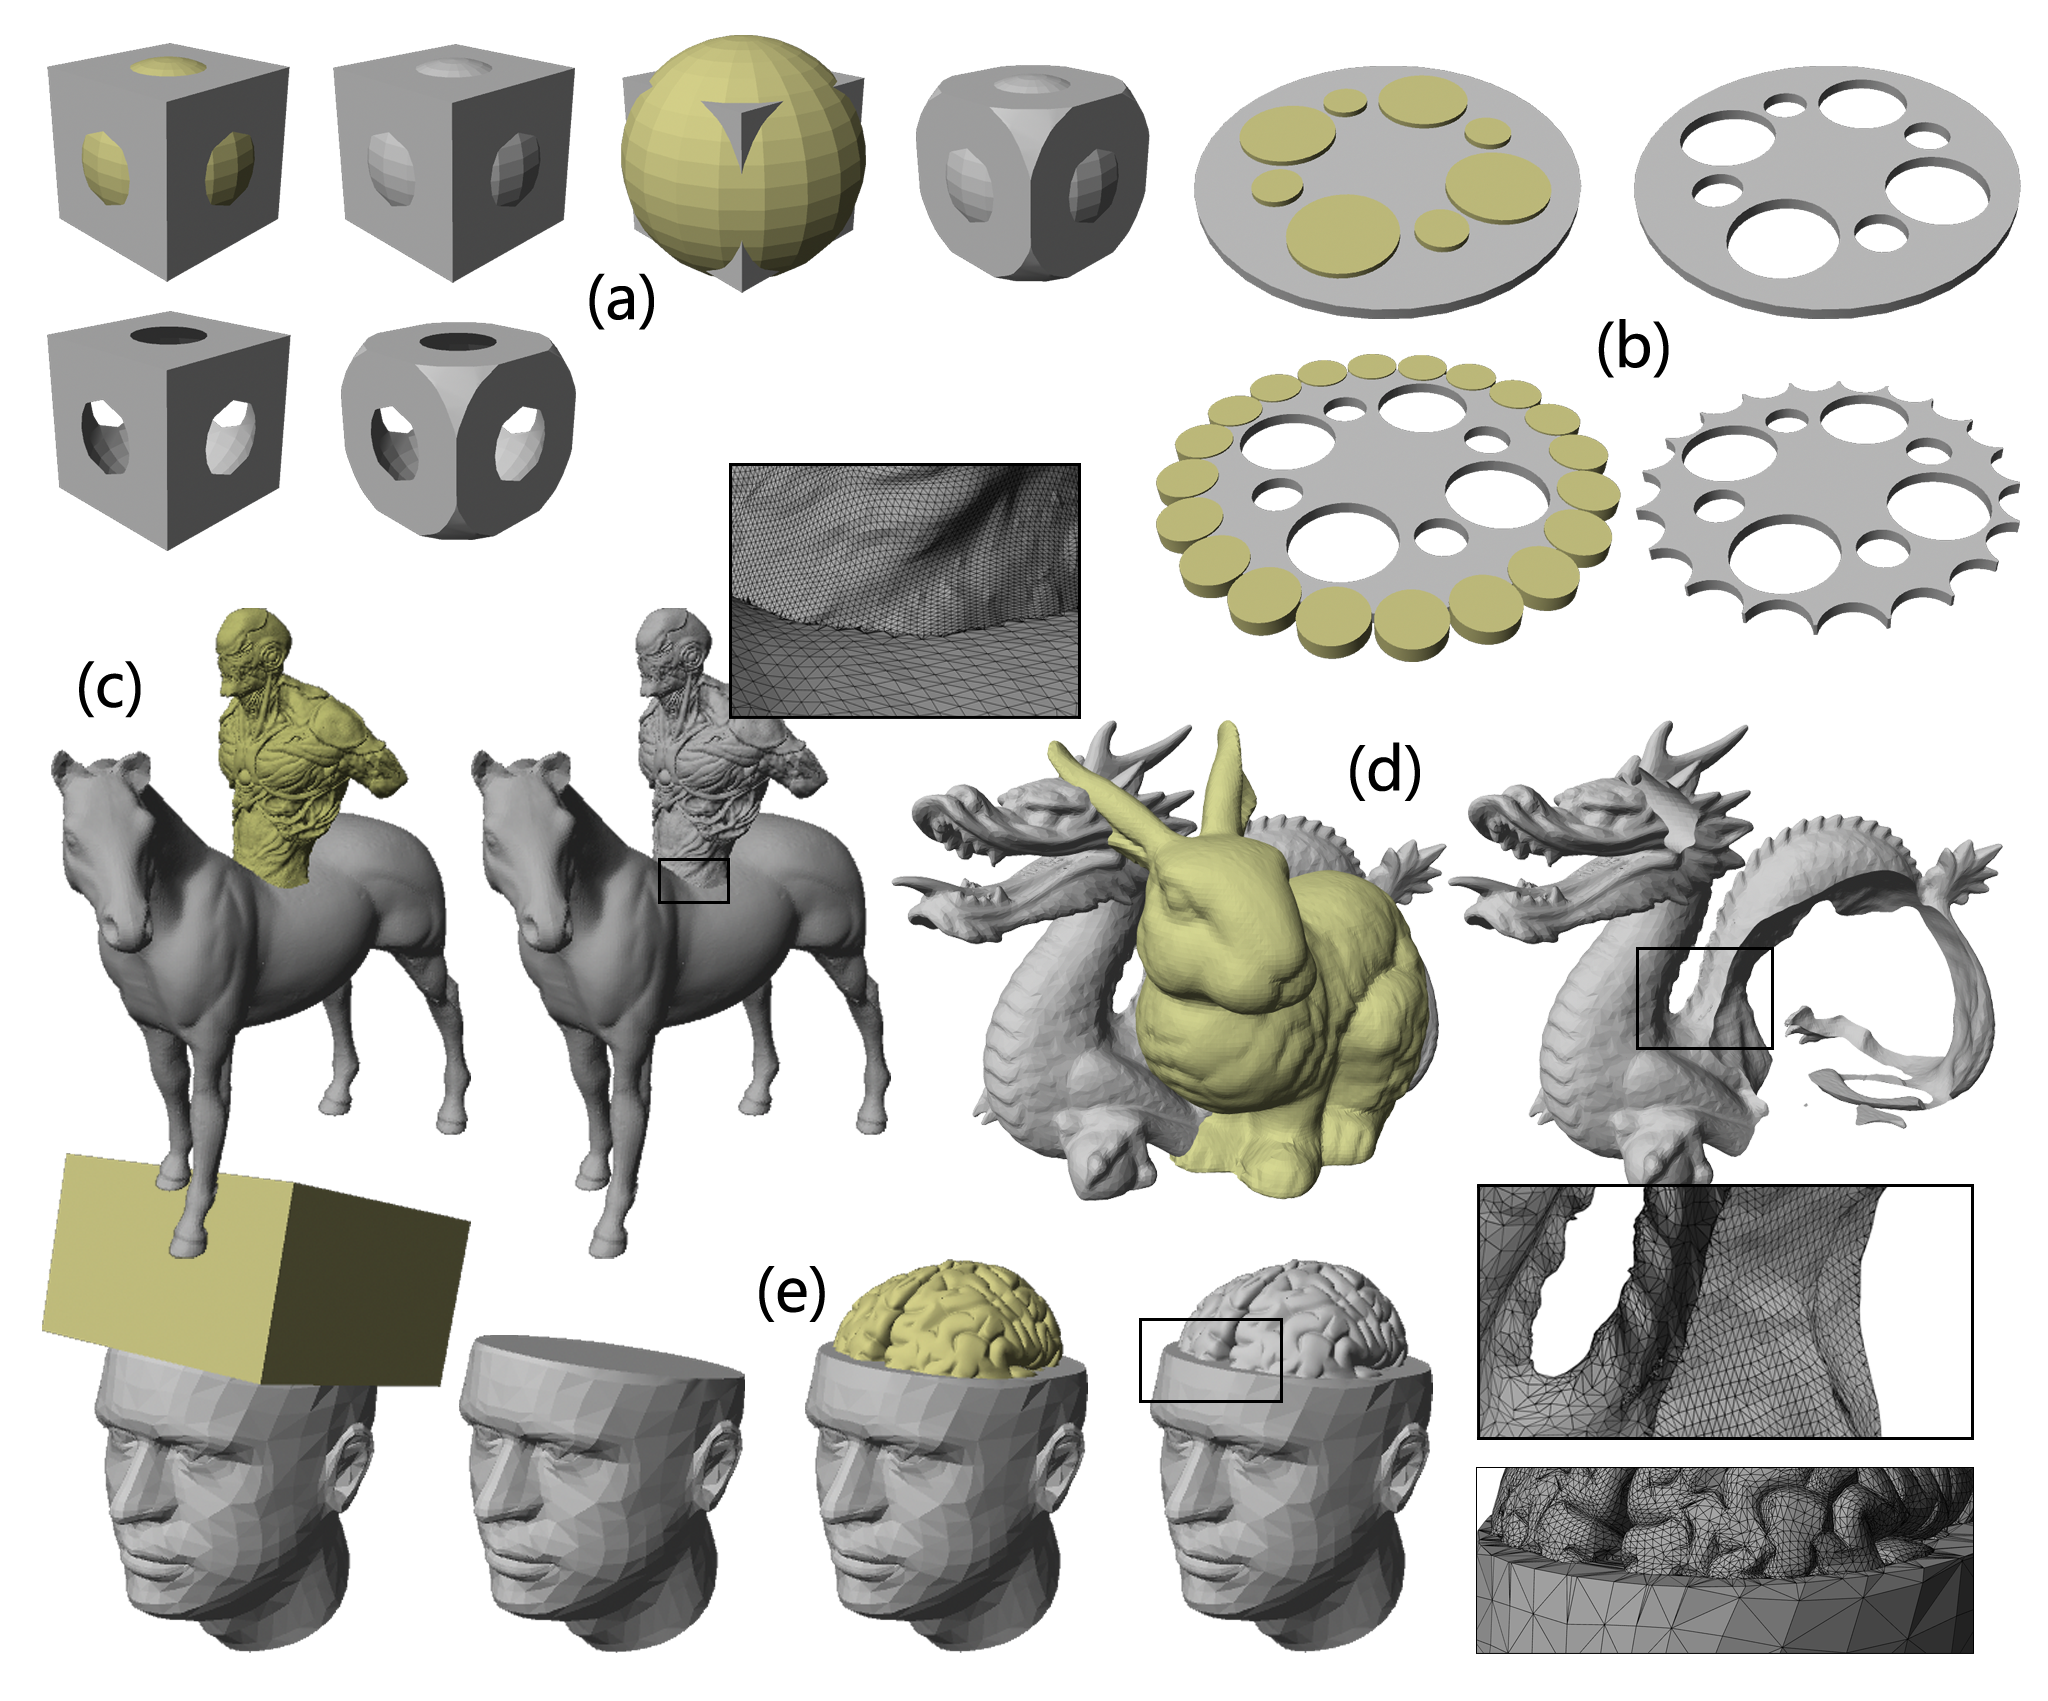
\includegraphics[width=7in]{models}
\caption{***********different models: will be replaced}
\label{fig:models}
\end{figure*}

\subsection{Implementation}
\label{sec:esubroutine}


\vspace{0.5em}
\noindent\textbf{Tess-graph with multiple components. }
There is no guarantee that the tess-graph will be a connected graph. If a tess-graph contains more than one connected component, we need to merge identical valid loops, which allows us to generate polygons with non-zero genus. To find identical loops, we construct an auxiliary connection $C_{ext}$ for each inner component, which connects a vertex $\bm{v}_o$ on the outer component and a vertex $\bm{v}_i$ on the current inner component (see Fig. \ref{fig:dual}a). After that, we search all the connections belongs to the current inner component that intersection $C_{ext}$, and find the one (as $C_1$) which is the nearest to $\bm{v}_o$. Then we search all the connections not belongs to the current inner component that intersection $C_{ext}$, and find the one (as $C_2$) which is the nearest to $C_1$. Finally, by figuring out in which valid loops $C_1$ and $C_2$ are, we find the identical pair of loops.

To guarantee that $C_{ext}$ has an exact P-rep within double-precision, the vertex of triangle is chosen as the $\bm{v}_o$. On the other hand, $\bm{v}_i$ must be the vertex generated by the intersection between an triangle and an edge (as $\bm{e}$). All intersection points introduced by triangle-triangle intersections are of this type. In this way, we obtain three vertices with exact coordinates ($\bm{v}_o$ and the two end points of $\bm{e}$). Therefore, we can construct the plane on which $C_{ext}$ lies by the same method of generating supporting planes of triangle faces (see Fig. \ref{fig:dual}b).

\vspace{0.5em}
\noindent\textbf{Seed label generation. }
The label vector of the seed vertex $\bm{\Lambda}(\bm{v}_0)$ can be generated by a point-in-polyhedron test \cite{ogayar2005point}, using the octree as an acceleration structure \cite{frisken2002simple}. However, a simpler strategy can be adopted which chooses a vertex with known labels as the seed. The inclusion labels of vertex with the maximum $x$-coordinate are either $out$ ($in$, if the complement is applied on the mesh) or $on$. The $on$ labels can be determined by connectivity. Exceptions can occur because of our ignorance of coplanar situations---vertices may not be added to the primitive, even if they are on surface of it. Fortunately, if seed vertex is chosen whose neighboring faces are not all coplanar, exceptions can be avoided.

Label vectors can propagate within a certain mesh, and between different meshes across shared edges. Therefore, in most cases, only a single seed vertex is needed for classification. However, if there are more than two connected components among the tessellated meshes, extra seeds are required. The labels of these additional seeds have to be computed by point-in-polyhedron tests.

\vspace{0.5em}
\noindent\textbf{Exporting to float-point number. }
The vertices of the final mesh are represented as either planes or vertex coordinates. The vertices originating from the input meshes have exact coordinates, and the vertices newly introduced by the intersection between meshes have only P-reps, and require round-off when computing their coordinates. Although our method guarantees the correct topology in the final mesh, round-off errors can still cause topological deficiencies. This is called \textbf{vertex rounding} problem. We adopt the method of Zhou et al. \cite{zhou2016mesh} to solve this problem iteratively.

\subsection{Limitations and Future Work}

We found that performance of our method was poor for CSGs that contained a lot of meshes within a small area (Table. \ref{tab:performance}, \emph{T1}). In these cases, our method computes many intersections that will not appear as edges in the final mesh, leading to unnecessary tessellation. Optimization may be explored to alleviate this problem.

The inputs of our method are limited to solids. However, recent reports have proposed that the piece-wise wind number (PWN) is a more powerful method to identify the insides and outsides of meshes \cite{zhou2016mesh}. The input requirements of our method may be extended to PWN meshes, that allow self-intersection. We believe that this would be an interesting and valuable extension of our work.

\section{Summary}

In this paper, we propose a novel boolean method. Our method can efficiently perform variadic boolean operations, and is robust with solid inputs. The novel component of our approach is to combine P-reps with V-reps. P-reps allow us to strictly follow the principle of no geometry construction to avoid numerical errors ,and the V-reps enables coarse tests and fast neighborhood queries to reduce the need of slow plane-based computation. The experimental results show that the performance of our method is competitive with state-of-the-art non-robust methods, while guaranteeing robustness under consistent inputs.
